 %!TEX root = Memoria_TFM.tex
\section{Anti-spoofing and biometrics systems}
At the same time that technology has evolved, capture systems and processing algorithms have proceeded too. This opens up a wide variety of options,  one of them being the capability of developing biometrics systems, giving way to identification and recognition systems.\\

A biometric system is a software and hardware system which is based on human physical characteristics or psychological behavior in order to identify a person.

\subsection{Historical introduction}
It was in the 1870s when the necessity of identifying people by getting physical characteristics appeared. Alphonse Bertillon had the desire to identify jail prisoners, and in order to satisfy this need, the skull diameter, arm and foot length were used in the USA until the 1920s \cite{Intro_biometrics}.\\

It was back in the 1880s when fingerprint and facial identification were proposed. With the appearance of digital signals processing systems in 1960, voice and fingerprint biometric systems began to be investigated and researchers started to have the idea of using this system to identify people in access control security \cite{Intro_biometrics}.\\

Ten years later, the geometry of the hand commenced to be an area of interest for automated identification technologies. The retina and signature verification appeared in the 80s and after a short period of time, the face systems appeared too\cite{Intro_biometrics}.\\

The last biometrics systems appeared in the 1990s with the iris recognition \cite{Intro_biometrics}.

\subsection{Biometrics}
Biometrics refers to characteristics that humans own. These characteristics should be inherent and are exclusive to each human. Because of this, they are used for identification purposes.\\

Biometrics could be distinguished as physical or behavioral biometrics. Physical biometrics are characteristics which every human is born with and trey are purelt genetic, fingerprint, face, DNA, ear and iris are physical biometrics. Behavioral biometrics are characteristics that a person has developed, they are  psychological characteristics, signature and gait are behavioral biometrics \cite{biometrics_beha}.\\

Nowadays, the quantity of biometrics is considerable. There is not a biometric which is only used or could be selected as optimal, although fingerprints are the most popular biometrics \cite{2d_3d_face}. The characteristic of each biometrics makes it appropriate for each particular application \cite{Intro_biometrics}.\\% The most common biometrics are described \cite{Intro_biometrics}:

%\begin{description}[itemsep=2pt,topsep=8pt,parsep=0pt,partopsep=20pt] \item \textbf{DNA:} using the DNA for recognition is widely used in forensic. This biometric is intrusive and identical twins share the ADN \cite{Intro_biometrics}. \end{description}

%\subsubsection{Face biometric}
%The thesis research is focused on face biometric.\\

\subsection{Biometric system}
A biometric system could be defined as a structure which collects spefific biometric data from a user. The input data is processed in order to obtain features which are compared with template samples. A biometric system could be labeled as a recognition system or verification system depending on the task carried out\cite{Intro_biometrics2}:
\begin{description}[itemsep=2pt,topsep=8pt,parsep=0pt,partopsep=20pt]
\item \textbf{Verification system:} user claims an identity and the system validates the identity comparing the acquired data with the data stored in the template database. It is a one-to-one comparison.
\item \textbf{Recognition or Identification system:} user data is compared with the all the template database to find the user's identity. The identity is not claimed by the user and is given by the system according to the features. It is a one-to-all comparison.
\end{description}

\begin{figure}[htb]
\centering
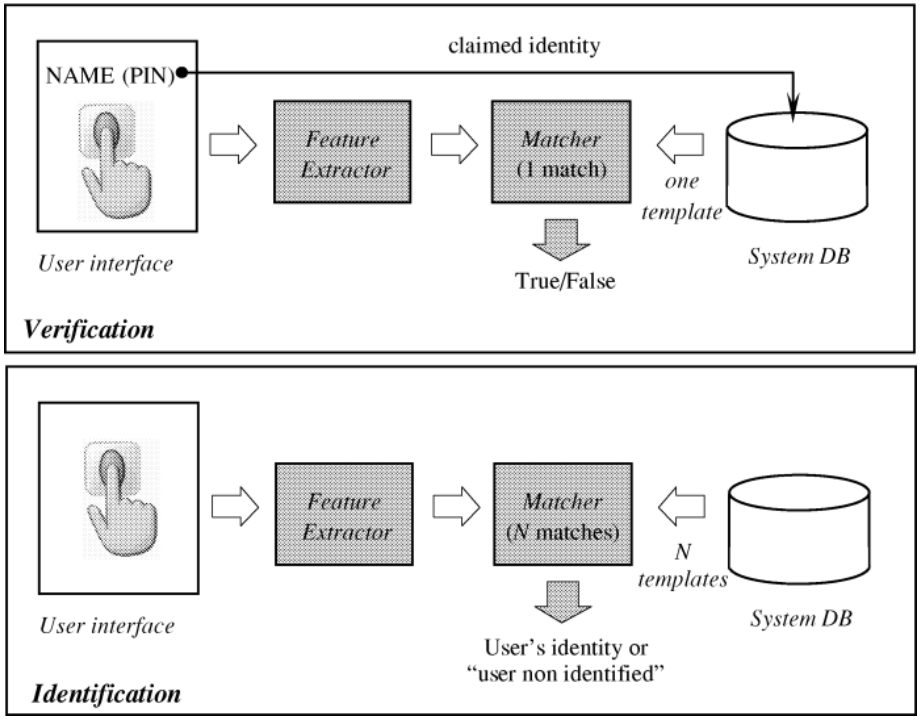
\includegraphics[width=0.5\textwidth]{images_miscelaneus/verif_identif.PNG}
\caption{Verification and Identification system diagram. Image obtained from \cite{Intro_biometrics2}.} \label{fig:Verif_ident}
\end{figure}

Figure \ref{fig:Verif_ident} (figure obtained from \cite{Intro_biometrics2}) briefly represents  the process of the acquired data until it is compared  with the system database to see if it is a verification or recognition system. The modules shown in figure \ref{fig:Verif_ident} are described \cite{Intro_biometrics2}:
\begin{description}[itemsep=2pt,topsep=8pt,parsep=0pt,partopsep=20pt]
\item \textbf{Sensor:} the first module is the sensor, which obtains the user's biometric. Depending on the biometrics, the sensor can vary greatly.
\item \textbf{Feature extractor:} input data is processed to obtain the features. The features that are extracted in this module should be the same as the one saved in the database.
\item \textbf{Matcher:} features obtained from the previous module are compared or classified with the templates database so that the identity of the user could be verified or assigned.
\item \textbf{Database:} the database is made by templates which are used as true samples to compare the ones obtained with the sensors. A user should be registered to the system contributing with its biometric template.
\end{description}

Some biometrics could be used at the same time, in the same biometrics system, by adding the biometrics in the feature or score level. It is labeled as multimodal and it is used to complement vulnerabilities of biometrics \cite{Spoofing_survey}.

\subsection{Spoofing}
At the same time that biometrics authentication systems appeared, the attacks to trick systems also emerged and they were called \textit{spoofing attacks}. For instance,making plaster molds for geometric hand biometrics or fingerprints would be an attack just like the one presented in figure \ref{fig:Spoof_fingerprint} (image obtained from \cite{fingerprint_image}).\\

\begin{figure}[htb]
\centering
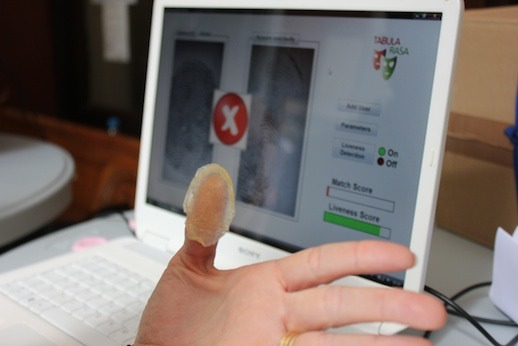
\includegraphics[width=0.5\textwidth]{images_miscelaneus/spoofing_fingerprint.jpg}
\caption{Spoofing fingerprint. Image obtained from \cite{fingerprint_image}.} \label{fig:Spoof_fingerprint}
\end{figure}

Spoofing is referenced to impersonate a biometric system trying to be verified or to get an identity when the user is not a genuine. The attack would depend on the biometry and the capturing system \cite{Spoofing_survey}. Attacks are usually made with artificial articles.\\

In order to identify the tricks and putting an end to  spoofing attacks, \textit{anti-spoofing} tries to minimize the attacks or prevent them.\\


Anti-spoofing methods could be distinguished depending on the biometric system module which is combined \cite{Spoofing_survey}:
\begin{description}[itemsep=2pt,topsep=8pt,parsep=0pt,partopsep=20pt]
\item[Sensor level:] extra equipment is added to the sensor, the new device is responsible for getting a living attribute as sweat or blood pressure.
\item[Feature level:] anti-spoofing detection is made after the sample has been acquired. The sample is processed and the software decides if it is a genuine or fake user.
\item[Score level:] after the feature extraction, when the scores are obtained, the biometric system decides if the user is genuine or not fusing methods. This method is the newest.
\end{description}

Anti-spoofing systems and scenarios could be evaluated. Depending on how they are evaluated, two methodologies are distinguished \cite{Spoofing_survey}:
\begin{description}[itemsep=2pt,topsep=8pt,parsep=0pt,partopsep=20pt]
\item[Algorithm-based or technology evaluation:] Evaluates algorithms that prevent anti-spoofing.
\item[System-based or scenario evaluation:] Evaluates the entire acquisition systems including the sensor.
\end{description}

In this project,  an algorithm is going to be developed so as to detect anti-spoofing attacks when the face is used as biometrics. Given an image, the system has to decide if it is an attack or a genuine user. It would be a verification task.

\subsection{Face anti-spoofing}
Face biometrics is a frequently used biometric system because of its attributes since it is not intrusive, it is easy capturing images and it is considerably accepted by people as biometrics. \\

The principal or main used acquire systems are visible light cameras, apart from, other cameras as infra-red or depth camera that can also be used too. Moreover, using different types of cameras could help to detect anti-spoofing attacks.\\

The disadvantages of cameras as sensors are that the illumination needs to be controlled and images from different angles may not always be be suitable. In addition, people’s expressions or face occlusions are complicated to work with \cite{survey2,2d_3d_face}. On the contrary, the main advantage of using a visible light camera as sensor is the cost, which is affordable. \\

The location of verification or identification systems could be in a static and specific place as the office entrance or a wide place as a subway or an airport \cite{survey2}.\\

The spoofing attacks could be 3D attacks, if 3D masks are used; printed photos; 2D mask and displaying an image or video on a smartphone or tablet can also be considered 2D attacks \cite{2d_3d_face}. The cost of 2D attacks is not high \cite{distorsion} and less expensive than 3D spoofing attacks.\\


\begin{figure}[htb]
\centering
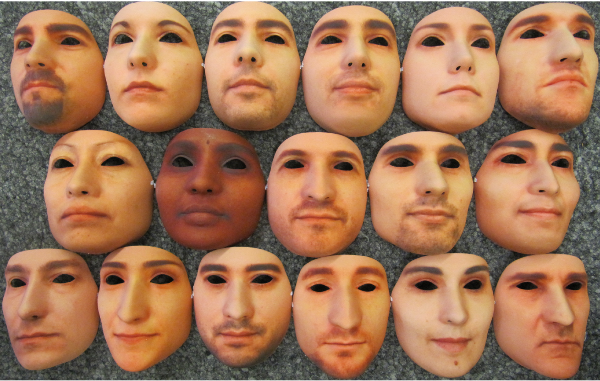
\includegraphics[width=0.5\textwidth]{images_miscelaneus/fig_masks.png}
\caption{3D face masks. Image obtained from \cite{3dmask}.} \label{fig:3dMasks}
\end{figure}

In figure \ref{fig:3dMasks} (image obtained from \cite{3dmask}) 3D resin face masks  are represented. These masks are used for a 3D face mask database, but are an example of face spoofing attacks. A 3D mask could be made of silicone too and is cheaper than a resin mask.\\

A 2D mask, printed photos or images and videos displayed on a smart device are attacks that easier to obtain thanks to the accessibility to personal information in social networks or the easy purchase of visible light cameras.\\


To discuss about spoofing attacks, the feature level is the most studied method. Literature separates it into two different groups: the dynamic and the static approach \cite{Spoofing_survey}:
\begin{description}[itemsep=2pt,topsep=8pt,parsep=0pt,partopsep=20pt]
\item[Dynamic:] it is based on motion to detect anti-spoofing. blinking eyes or optical flow assessment for example. Therefore, a temporal sequence of images are needed. It could be efficient when image attacks are used, but not too accurate when videos are used.
\item[Static:] a unique image is analyzed.
\end{description}

Different techniques to decide if a user is being impersonated or not are being researched and could be used with image and video sequences \cite{Spoofing_survey}.\\

Texture-based methods are one of the most investigated. Local Binary Patterns (LBP),  Histogram of Oriented Gradients (HOG) or Difference of Gaussian (DoG) are algorithms used to extract images features \cite{distorsion,Spoofing_survey}.\\

Motion or liveness detection methods search for movement in videos, asking the user to make a movement or analyzing the video frames sequence. The liveness could be detected in the blinking of the eyes, lip movement or head rotation \cite{distorsion,Spoofing_survey}.\\

Others methods, as multispectral-based anti-spoofing, use images obtained from an alternative to visible light cameras such as infra-red cameras \cite{distorsion}.\\

Generally, the explained methods work with 2D face anti-spoofing.  However, 3D anti-spoofing is present too used as sensor depth cameras \cite{2d_3d_face}. This thesis is focused on 2D face anti-spoofing.\\
